%!TEX root = paper.tex
\section{Related Work}
\label{sec:relatedwork}
%\todo{Move related work top}
\subsection*{BLE MAC-Layer Fingerprinting}
%
At its most basic level, BLE's design frustrates MAC-layer fingerprinting.
%
Although BLE advertisements contain a full 6-byte MAC address that is unique to the
advertising device, the BLE protocol also has built-in cryptographic MAC randomization.
%
Fortunately, prior work found (and we confirmed) that mobile devices are
properly implementing BLE's MAC address randomization~\cite{Iphonetracking_becker,MACRandomizationfail_Martin}.
%
Namely, they found devices are following the BLE specification and periodically
(every 10--15 minutes) randomizing their MAC addresses~\cite{bluetoothprivacy}.
%

However, several papers have performed privacy attacks by deriving identifiers from the packet contents of beacons that were not reset properly after the MAC was
randomized, for both WiFi~\cite{sn1,MACRandomizationfail_Martin} and BLE~\cite{ryanble,spill2007bluesniff,Iphonetracking_becker,HandoffMartin,celosia2020close} radios.
%
However, all of these attacks fall short as they either require the receiver to continuously listen to beacons from the target devices, or fundamentally rely on identifiers that can easily be removed through simple software updates.
%
This limits the attacker's ability as they must persistently follow a target to track it.
%
Thus, link layer techniques don't provide persistent identifiers that can be utilized for long term tracking of devices.

\vspace{0.5em}

\subsection*{Physical-layer Fingerprinting}

\begin{figure}[t!]
    \centering
    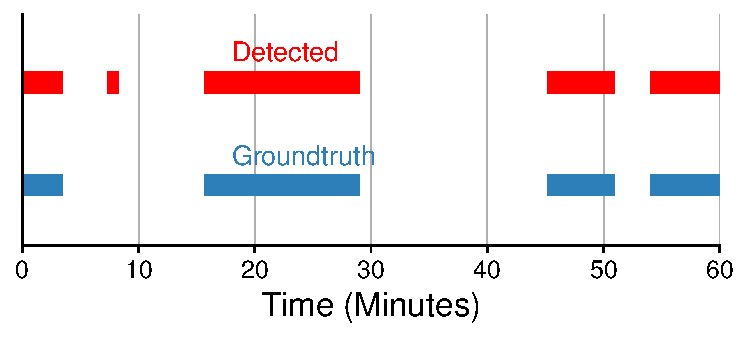
\includegraphics[width = 0.9\linewidth]{bletracking/plots/case_study_android2.pdf} 
    \caption{The blue bar represents the time that the target was present, the red bar represents the time that our tracking toolkit detected the presence of the target.}
    \label{fig:android}
\end{figure}

RF fingerprinting using hardware impairments is a well studied field.
%
Researchers have analyzed various hardware impairment based signal properties such as CFO, \iq offset/imbalance, signal transients and others~\cite{Brik_radiometric,vohuuusrp,Intrusion_hall,deviceID_kose,suskitransient,roguewifi_liu,oscillator_azamehr}, and leveraged various statistical methods, and in recent times deep learning approaches~\cite{gopalakrishnan2019robust,denoising_yu,deeplearning_merchant} to fingerprint these properties. For instance, the transient portion of the signal has been proposed as a unique signature to 
classify different wireless devices~\cite{extraction_rehman, transientID_danev} even Bluetooth
signals~\cite{transientBT_Hall}. However, the transient portion of BLE and Bluetooth signals
is only about 2 microseconds and contains insufficient information to uniquely identify 
a device among tens of devices. Modulation-shape features have also been explored for RF
fingerprinting devices such as RFID transponders~\cite{rfidphysical_danev}. However, 
the Gaussian shape in GFSK modulation of BLE signals is generated digitally in most 
personal electronic devices such as phones, and thus, cannot be used as a unique fingerprint.
In the WiFi literature, CFO and \iq imperfections (\iq origin offset and \iq imbalance) are 
two well recognized features which have been shown to be the most separable features for 
WiFi fingerprinting~\cite{Brik_radiometric}. 

BLE hardware in mobile devices are similar in architecture and suffer from the same hardware impairments as WiFi radios.
%
Despite that, other than a few efforts at coarse CFO extraction utilizing specialized hardware (CC2400)~\cite{cvtracksun,blueshieldjain}, there exists limited work in RF fingerprinting of these BLE chipsets. 
%
This is primarily because the techniques to extract these properties rely upon the presence of long known sequence of bits and pilots, a convenience not provided in simple BLE transmissions.
%
Even if the WiFi techniques were utilized for BLE signals, they would yield coarse estimates of these persistent identifiers, which are not particularly useful when fingerprinting a large amount of devices.
%
Furthermore, to be able to utilize any RF fingerprinting technique as a privacy attack, we need to have evidence that it works in real world settings. 
%
Unfortunately, all prior work in RF fingerprinting has been performed in controlled environmental settings with a defined set of devices. 
%
We design a technique to extract the hardware impairments such as CFO and \iq offset from BLE signals at a fine granularity. We were then able to collect a massive dataset of BLE devices in the wild and analyze their RF fingerprints to evaluate the potentials and limitations of the physical-layer fingerprinting privacy attack in the wild. We also demonstrated the feasibility of a location privacy (tracking) attack utilizing these physical-layer parameters in a realistic scenario.







